%% this is /book/ioos.txt
\section{Deploying \sciwms{} for the U.S. \ioos{} \comt{} Testbed}

The U.S. Integrated Ocean Observing System (\ioos{}) Coastal and Ocean
Modeling Testbed (\comt{}) was formed to unify otherwise disparate
entities in government, academia and industry to leverage the
proliferation of oceanagraphic data and modeling techniques to combat
natural and man-made coastal stressors by accelerating the turnaround
from research and development to operational application of
society-critical applications including: forecasting, model
comparison, model skill assessment, and algorithmic/parameterization
improvements~\cite{luettich13}. A crucial component for the success of
the U.S. \ioos{} \comt{} mission is a web accessable tool for quickly
visualizing and assessing a diverse set of coastal modeling
data. While \sciwms{} is a general software solution for geospatial
visualization, it is a key component in realizing the U.S. \ioos{}
\comt{} mission, facilitating qualitative model comparisons and
aggregation through a unified visualization framework.

\begin{figure}[ht!]
  \centering
  \includegraphics[width=0.6\columnwidth]{../figs/sciwms_overview_v2.pdf}
  \caption{Overview of the \sciwms{} deployment for the U.S. \ioos{}
    \comt{} project. \Sciwms{} updates its topology and endpoint
    database via a nightly service which queries CF-Compliant datasets
    cataloged by \ngdc{}. Model data is hosted on an external web server
    exposed by an \ncml{} facade as a single \netcdf{} data structure
    accessable to \sciwms{} via \opendap{}. \Sciwms{} responds to http
    clients interfacing through a custom built web portal.}
  \label{fig:overview1}
\end{figure}
\begin{figure}[ht!]
  \centering
  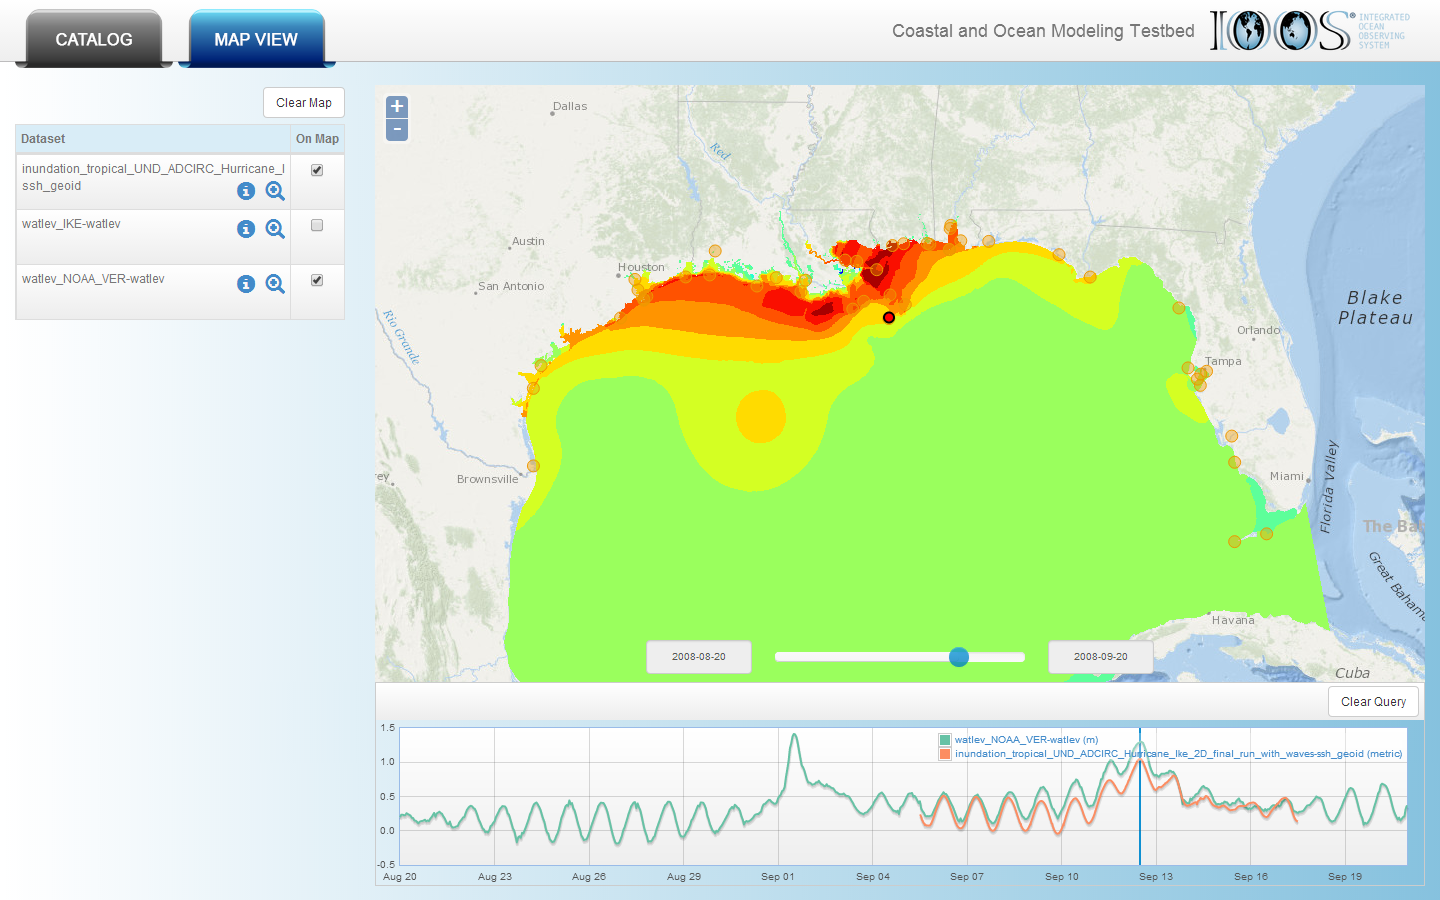
\includegraphics[width=0.8\columnwidth]{../figs/SciWMS_ModelObsComparison}
  \caption{Comparison of ADCIRC (unstructured topology) model results
    with observed water levels in the Northern Gulf of Mexico for
    Hurricane Ike. Verified observed water levels are from NOAA's
    Station 8760922 (red dot on map). The map shows modeled water
    levels (in meters above the geoid) at the peak of the storm in
    southern Louisiana. The time series plot shows both the modeled
    (green) and observed (orange) water levels. The vertical blue line
    in the time series plot corresponds to the current time of the
    map.}
  \label{fig:adcirc_comp}
\end{figure}

%% \begin{figure}[ht!]
%%   \centering
%%   \begin{subfigure}[t]{0.6\textwidth}
%%     \centering
%%     \includegraphics[width=\columnwidth]{../figs/sciwms_overview_v2.pdf}
%%     \caption{Overview of the \sciwms{} deployment for the U.S. \ioos{}
%%       \comt{} project. \Sciwms{} updates its topology and endpoint
%%       database via a nightly service which queries CF-Compliant datasets
%%       cataloged by \ngdc{}. Model data is hosted on an external web server
%%       exposed by an \ncml{} facade as a single \netcdf{} data structure
%%       accessable to \sciwms{} via \opendap{}. \Sciwms{} responds to http
%%       clients interfacing through a custom built web portal.}
%%   \label{fig:overview1}
%%   \end{subfigure}
%%   \begin{subfigure}[t]{0.6\textwidth}
%%     \centering
%%     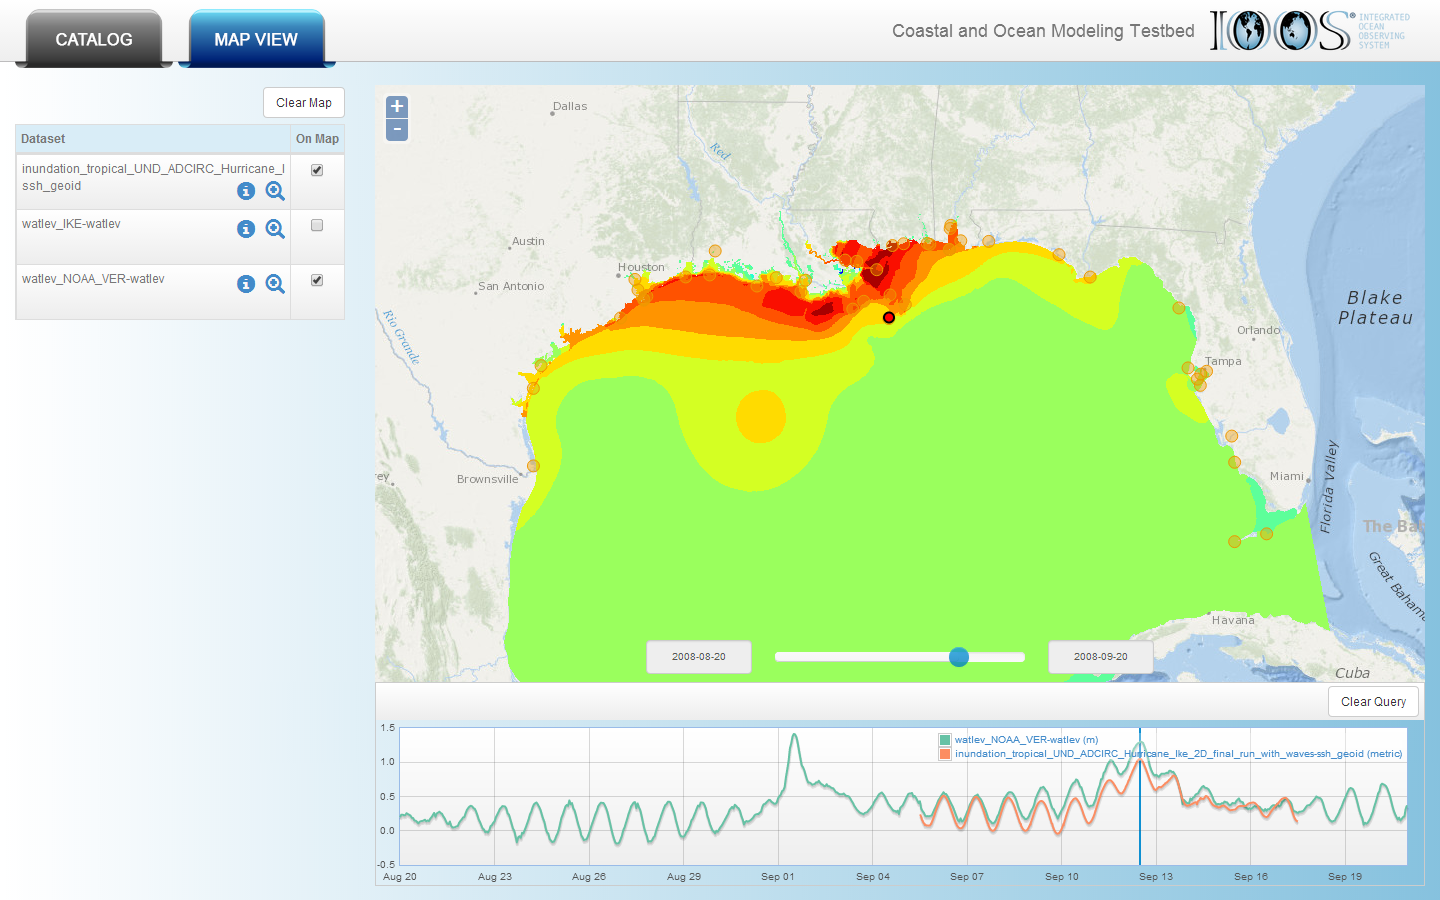
\includegraphics[width=\columnwidth]{../figs/SciWMS_ModelObsComparison}
%%     \caption{Comparison of ADCIRC (unstructured topology) model results
%%       with observed water levels in the Northern Gulf of Mexico for
%%       Hurricane Ike. Verified observed water levels are from NOAA's
%%       Station 8760922 (red dot on map). The map shows modeled water
%%       levels (in meters above the geoid) at the peak of the storm in
%%       southern Louisiana. The time series plot shows both the modeled
%%       (green) and observed (orange) water levels. The vertical blue line
%%       in the time series plot corresponds to the current time of the
%%       map.}
%%     \label{fig:adcirc_comp}
%%   \end{subfigure}
%% \end{figure}
%% \begin{figure}[ht!]
%%   \centering
%%   \includegraphics[height=2in]{../figs/sciwms_overview_v2.pdf}
%%   \caption{Overview of the \sciwms{} deployment for the U.S. \ioos{}
%%     \comt{} project. \Sciwms{} updates its topology and endpoint
%%     database via a nightly service which queries CF-Compliant datasets
%%     cataloged by \ngdc{}. Model data is hosted on an external web server
%%     exposed by an \ncml{} facade as a single \netcdf{} data structure
%%     accessable to \sciwms{} via \opendap{}. \Sciwms{} responds to http
%%     clients interfacing through a custom built web portal.}
%%   \label{fig:overview1}
%% \end{figure}
Figure~\ref{fig:overview1} outlines the cyberinfrastructre behind the
deployment of \sciwms{} for the \comt{}
project\footnote{\url{http://testbedwww.sura.org/explorer/}}. The
National Oceanic and Atmospheric Administration (\noaa{}) - National
Geophysical Data Center (\ngdc{}) geoportal indexes public geophysical
datasets and provides an \ogc{} \csw{} service to query datasets by
their metadata attributes. \sciwms{} queries the \ngdc{} Geoportal at
regular intervals updating the local topology cache and
structure-endpoint database
(figure~\ref{fig:sciwms_topology_endpoints}) with new or modified
datasets. Raw coastal data is hosted by the Southeastern Universities
Research Association (\sura{}) on a dedicated server for the \comt{}
project~\cite{luettich12}. Each data set may consist of multiple files
in different formats, and may be the result of very different models
run by various institutions with disparate computing
resources. However, accompanying each dataset is an \ncml{} virtual
layer which exposes each dataset as a single \netcdf{}~\cite{netcdf},
\opendap{}~\cite{Cornillon03} accessible object. Furthermore, the
\ncml{} facade presents a consistent set of meta information in
accordance to CF-Conventions~\cite{cf} providing services like
\sciwms{} access to the raw data through a uniform interface.

Currently, \Sciwms{} is used to visualize data from the first phase
groups of \ioos{} \comt{} program: {\em estuarine hypoxia, shelf
  hypoxia and coastal inundation}~\cite{luettich13}. For each modeling
group, \sciwms{} successfully generates consistent visualizations of
data generated by \adcirc{}~\cite{adcirc}, \fvcom{}~\cite{chen06},
\selfe{}~\cite{zhang08} and \slosh{}~\cite{chen84} coastal modeling
algorithms and serves as a use-case for how \sciwms{} can be leveraged
as a scalable solution for delivering visualizations of
scientific data to a diverse community.

\sciwms{} currently supports contour and filled-contour visualizations
styles for scalar attributes while 2D flow fields can be shown as
arrows or barbs for vector valued
attributes. Figure~\ref{fig:adcirc_comp} shows a web portal utilizing
the \sciwms{} backend to compare ADCIRC model output for Hurricane Ike
with water levels observed by \noaa{} stations and
figure~\ref{fig:vims_selfe_chesapeake} visualizes current direction
and speed in the Chesapeake Bay area. Figure~\ref{fig:vims_selfe_ssh}
renders the sea surface wave height computed along the Atlantic coast
of South America, the Gulf of Mexico, up to Canada. The topology in
this example is unstructured (\ugrid{}), a triangulation containing
over 5 million vertices (sample locations). Attributes are fetched
from the appropriate external server as needed, rendered, cached for
performance, but ultimately discarded after processing to minimize
storage redundency. Ongoing development is in progress for \sciwms{}
to support emerging geophysical datasets such as ensemble model output
and to provide clear visual support for the assessment and
quantification of model skill and performance metrics.
\begin{figure}[ht!]
  \centering
  \begin{subfigure}[t]{0.49\columnwidth}
    \centering
    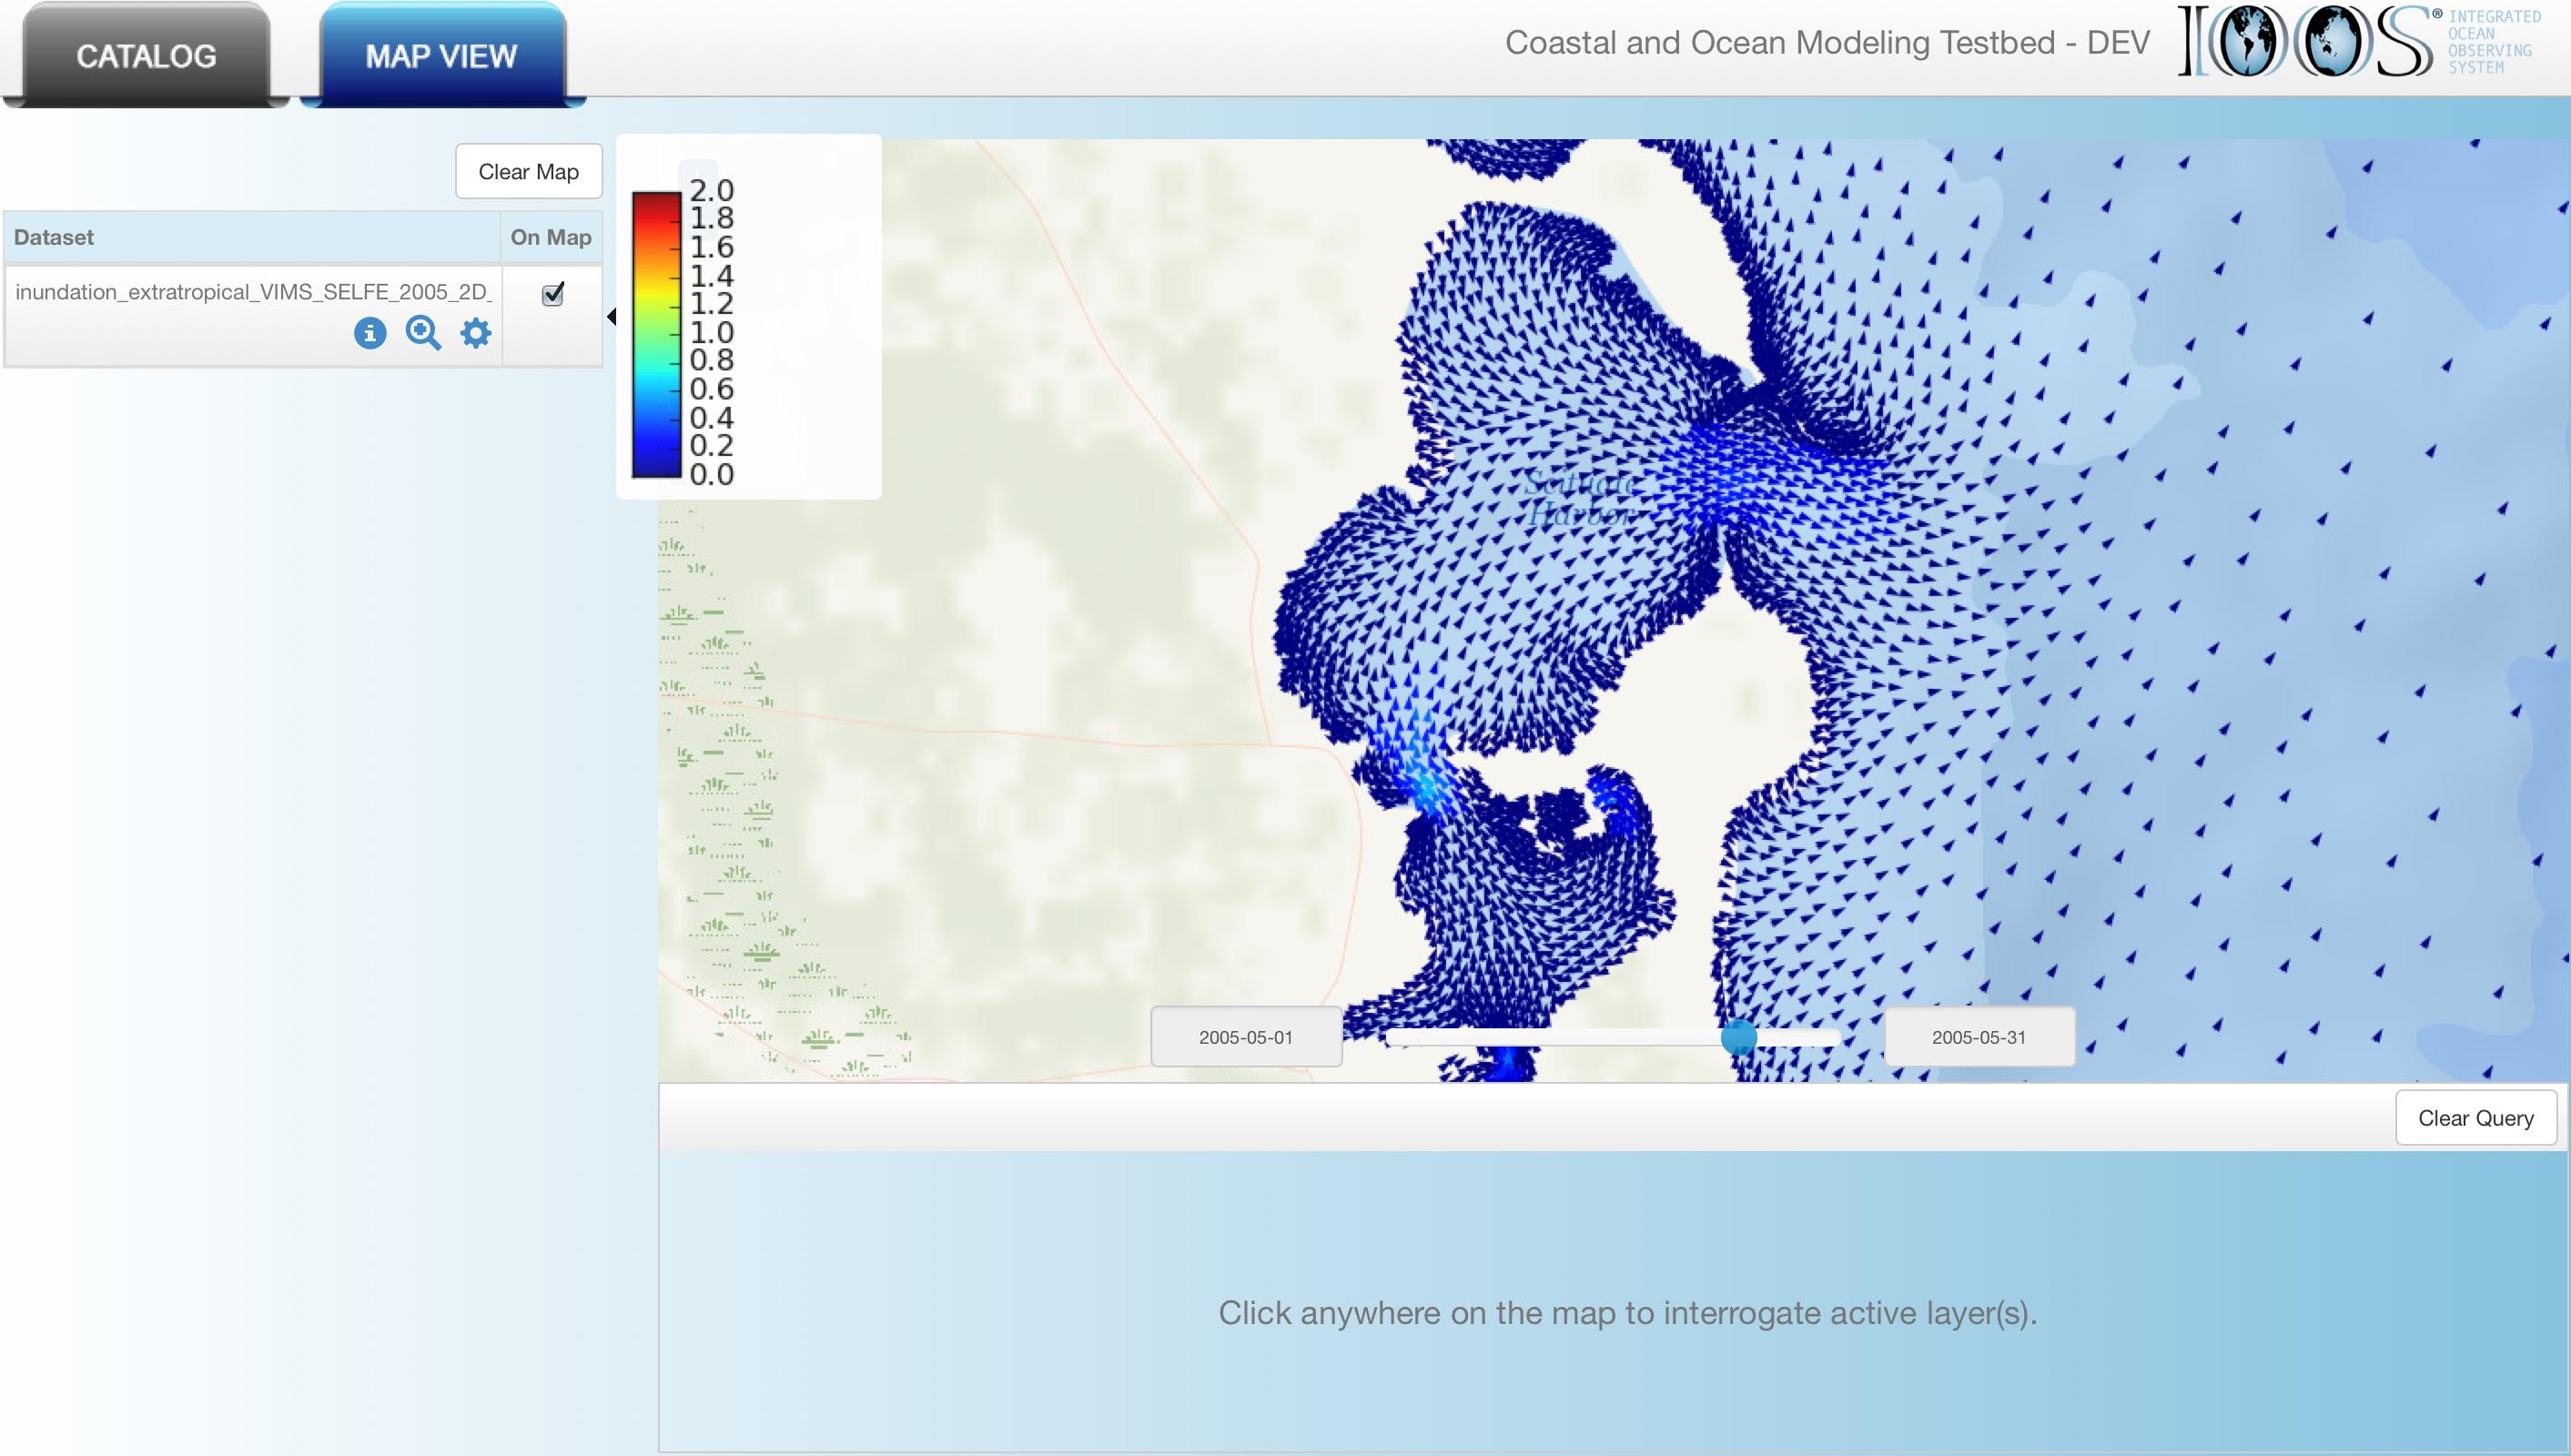
\includegraphics[width=\columnwidth]{../figs/vims_selfe_ubaratropic_vbaratropic_chesapeake_bay_crop_27_175_2825_1600}
    \caption{}
    \label{fig:vims_selfe_chesapeake}
  \end{subfigure}
  \begin{subfigure}[t]{0.49\columnwidth}
    \centering
    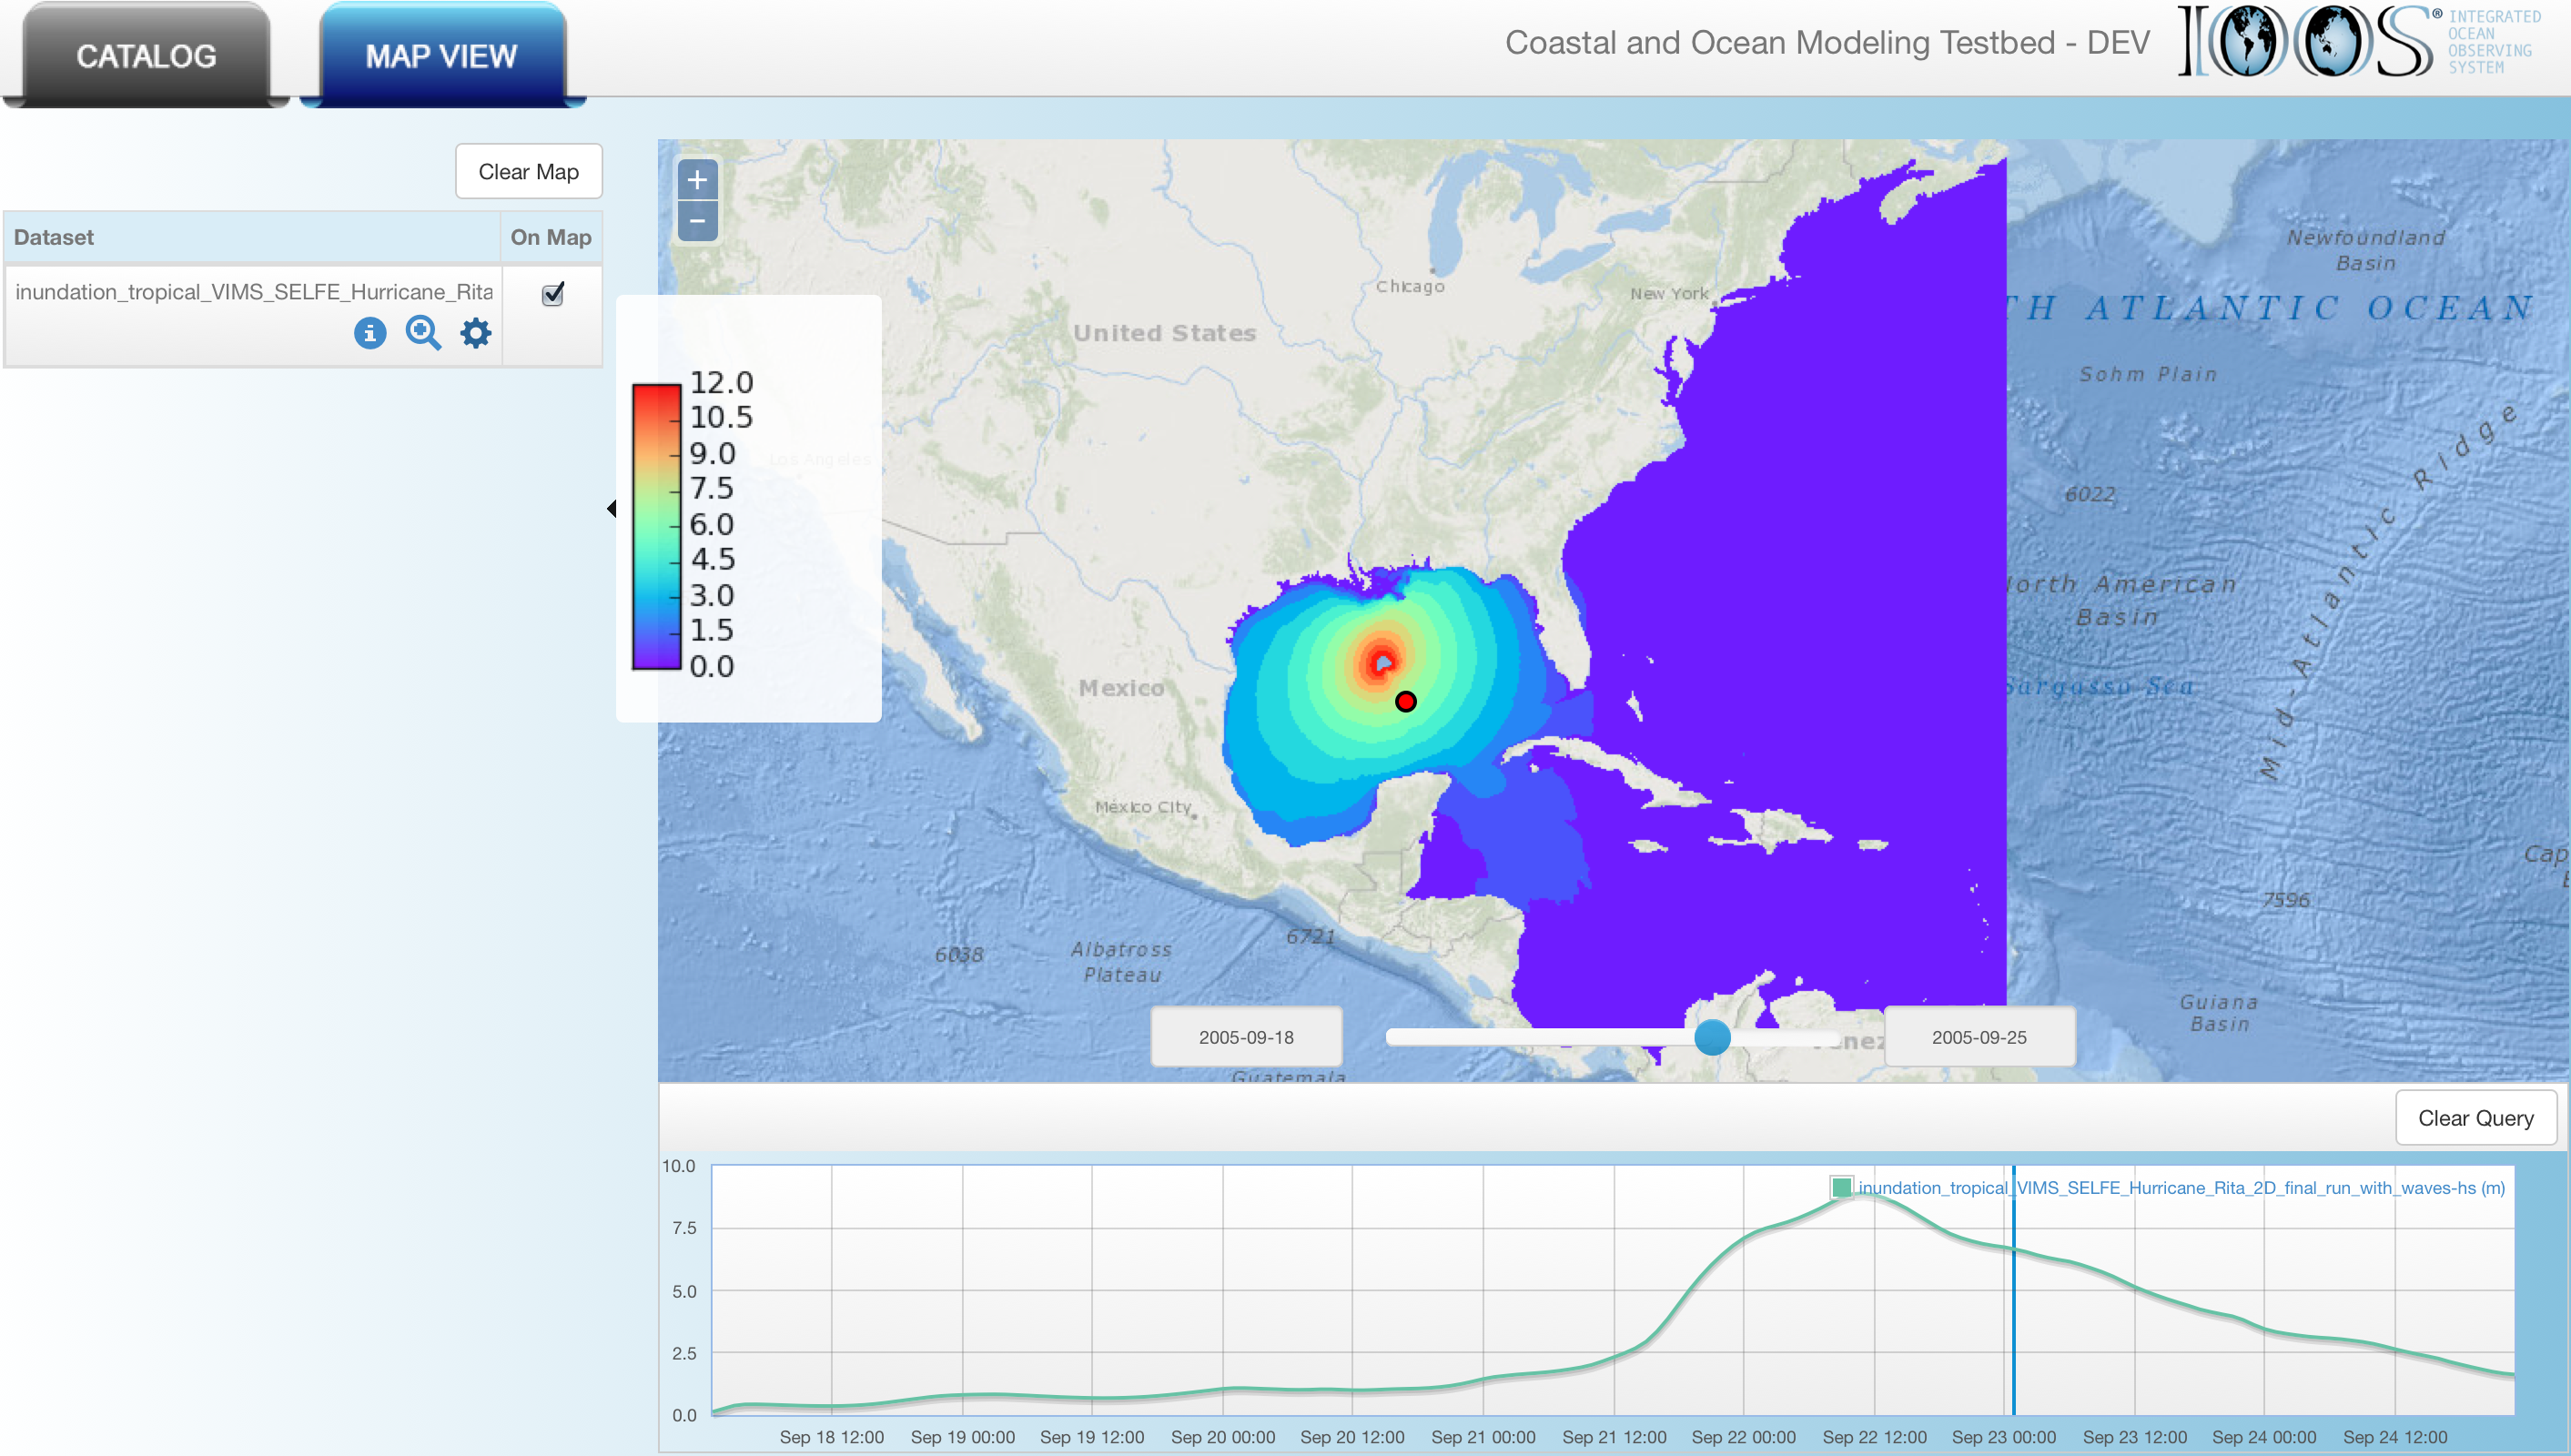
\includegraphics[width=\columnwidth]{../figs/inundation_tropical_VIMS_SELFE_hurricane_rita_2d_final_run_with_waves_sea_surface_wave_significant_height_crop_27_175_2825_1600}
    \caption{}
    \label{fig:vims_selfe_ssh}
  \end{subfigure}
  \caption{(a) Visualizing Current direction and speed in the
    Chesapeake Bay area. (b) Visualizing significant sea surface wave
    height along the eastern coast of the United States.}
\end{figure}
\FloatBarrier
